\documentclass{beamer}

\usepackage{HSE-theme/beamerthemeHSE}

\usepackage[english,russian]{babel}
\usepackage{fontspec}
\defaultfontfeatures{Ligatures={TeX},Renderer=Basic}  % свойства шрифтов по умолчанию
\setmainfont[Ligatures={TeX,Historic}]{Myriad Pro} %  установите шрифты Myriad Pro или (при невозможности) замените здесь на другой шрифт, который есть в системе — например, Arial
\setsansfont{Myriad Pro}  %  установите шрифты Myriad Pro или (при невозможности) замените здесь на другой шрифт, который есть в системе — например, Arial
\setmonofont{Courier New}
\uselanguage{russian}
\languagepath{russian}
\deftranslation[to=russian]{Theorem}{Теорема}
\deftranslation[to=russian]{Definition}{Определение}
\deftranslation[to=russian]{Definitions}{Определения}
\deftranslation[to=russian]{Corollary}{Следствие}
\deftranslation[to=russian]{Fact}{Факт}
\deftranslation[to=russian]{Example}{Пример}
\deftranslation[to=russian]{Examples}{Примеры}

\usepackage{multicol} 		% Несколько колонок
\graphicspath{{images/}}  	% Папка с картинками

\title[Заголовок]{\large Разработка системы контроля и управления энергопотреблением элементов графического интерфейса на мобильных устройствах \vspace{-2ex}}
\author[Юндин Владислав]{\footnotesize Юндин Владислав Андреевич\\ \vspace{2ex} Руководитель: Ролич Алексей Юрьевич, Старший преподаватель ДКИ\\ Соруководитель: Восков Леонид Сергеевич, профессор-исследователь, к.т.н., доцент}
\institute[Высшая школа экономики]{НИУ ВШЭ, Информатика и вычислительная техника}
\date{10 июня 2020 г.}

\begin{document}
    \frame[plain]{\titlepage}
    
    \begin{frame}
    	\frametitle{Введение}
        Проблема энергопотребления мобильных устройств становится всё более актуальной.\\~

        Цель: разработка системы контроля и управления энергопотреблением элементов графического интерфейса на устройствах под управлением операционной системы Android.\\~

        Задачи:
        \begin{itemize}
            \item Анализ;
            \item Выбор методологии измерения;
            \item Сбор данных;
            \item Создание библиотеки;
        \end{itemize}

    \end{frame}
    \begin{frame}
        \frametitle{Существующие решения}
        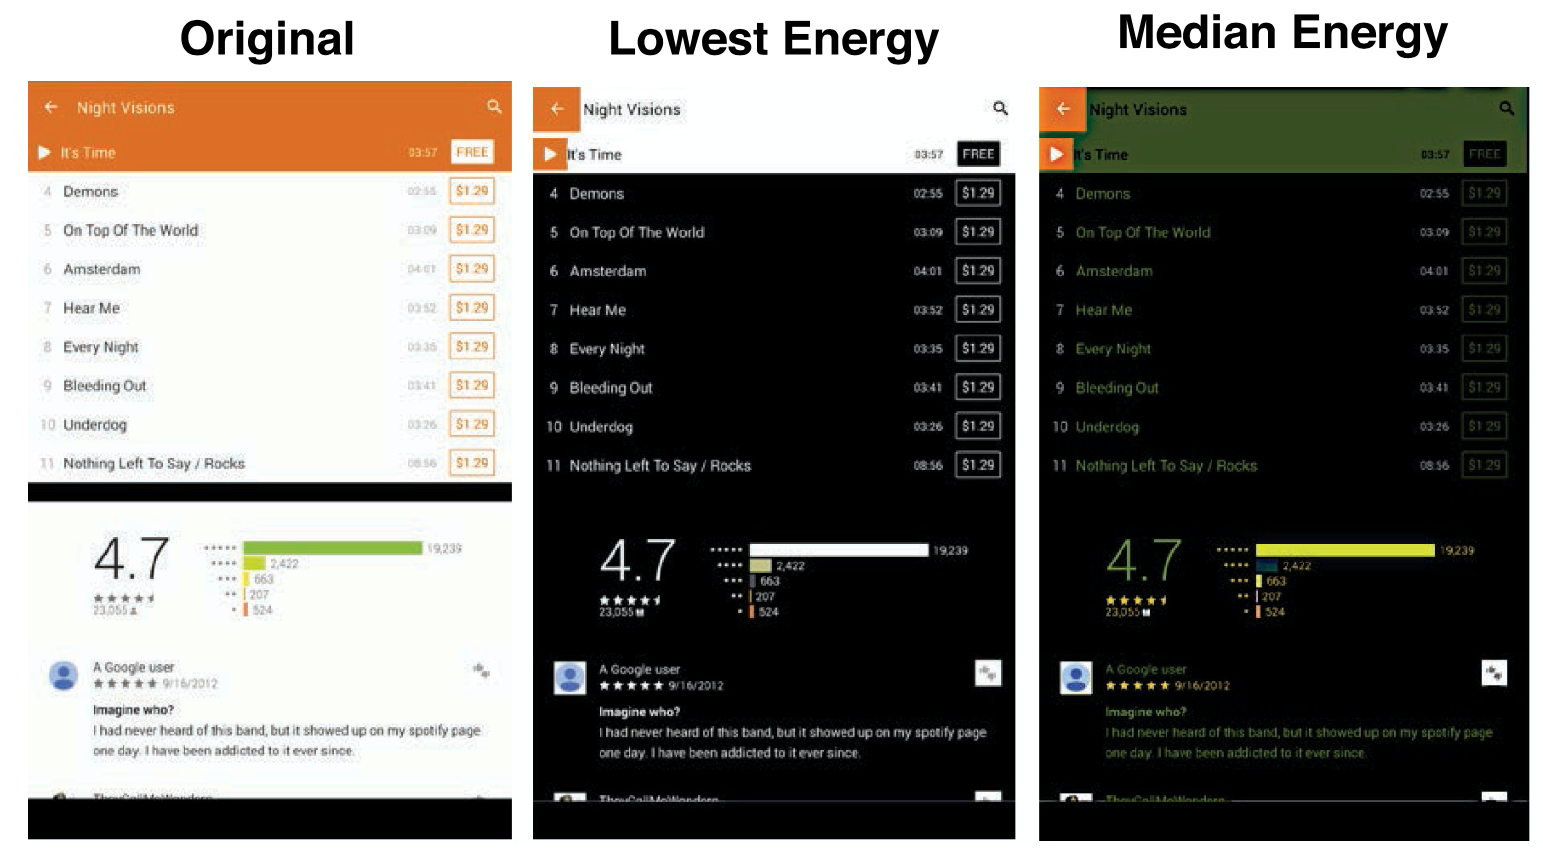
\includegraphics[width=\linewidth]{AMOLED}
    \end{frame}
    \begin{frame}
        \frametitle{Методология измерений}
        Способы измерений:
        \begin{itemize}
            \item Анализ напряжения, получаемого через BroadcastReceiver;
            \item Анализ данных Android Profiler;
            \item Анализ данных энергопотребления, получаемых через ADB;
            \item Анализ данных напряжения, получаемых через ADB;
            \item Использование стороннего оборудования;
        \end{itemize}~\\
        Были созданы инструменты сбора и анализа данных операционной системы.
    \end{frame}
    \begin{frame}
        \frametitle{Методология измерений}
        \framesubtitle{Влияние подключенного USB-кабеля}
        \begin{center}
            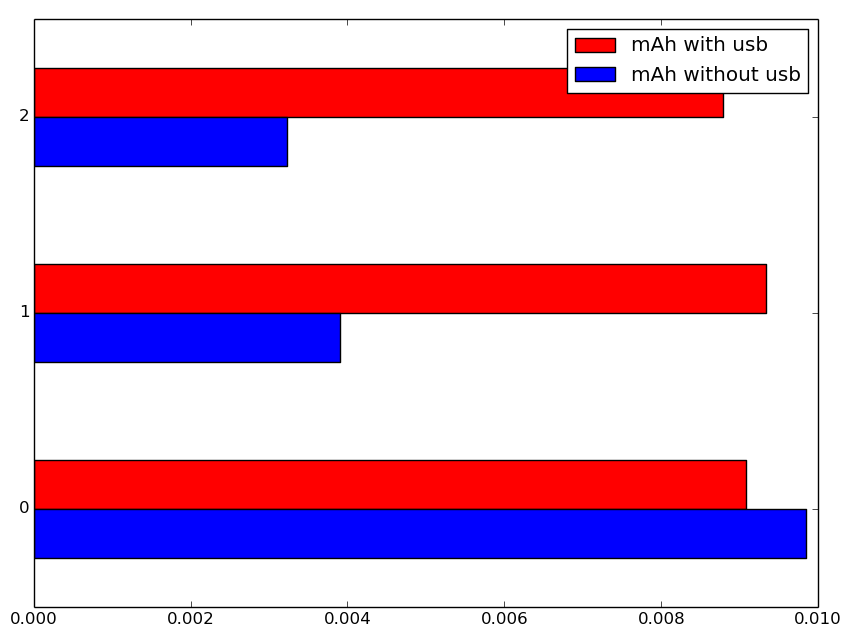
\includegraphics[width=0.9\linewidth]{usb_comparation}
        \end{center}
    \end{frame}
    \begin{frame}
        \frametitle{Методология измерений}
        \framesubtitle{Влияние запуска через автоматический тест}
        \begin{center}
            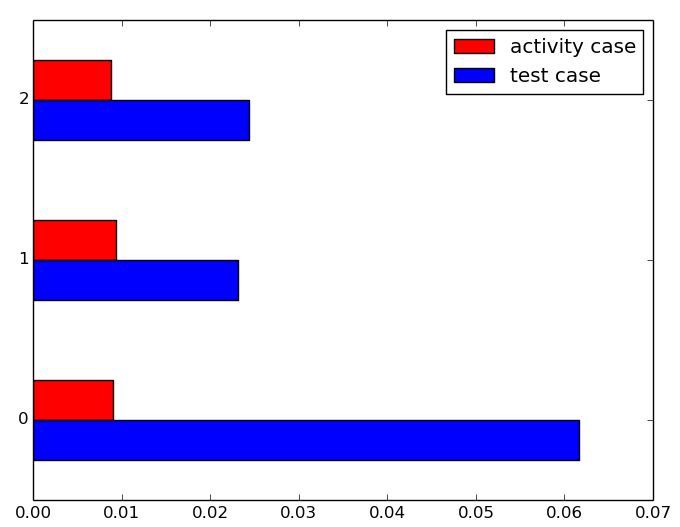
\includegraphics[width=0.8\linewidth]{test_comparation}
        \end{center}
    \end{frame}
    \begin{frame}
        \frametitle{Результаты измерений}
        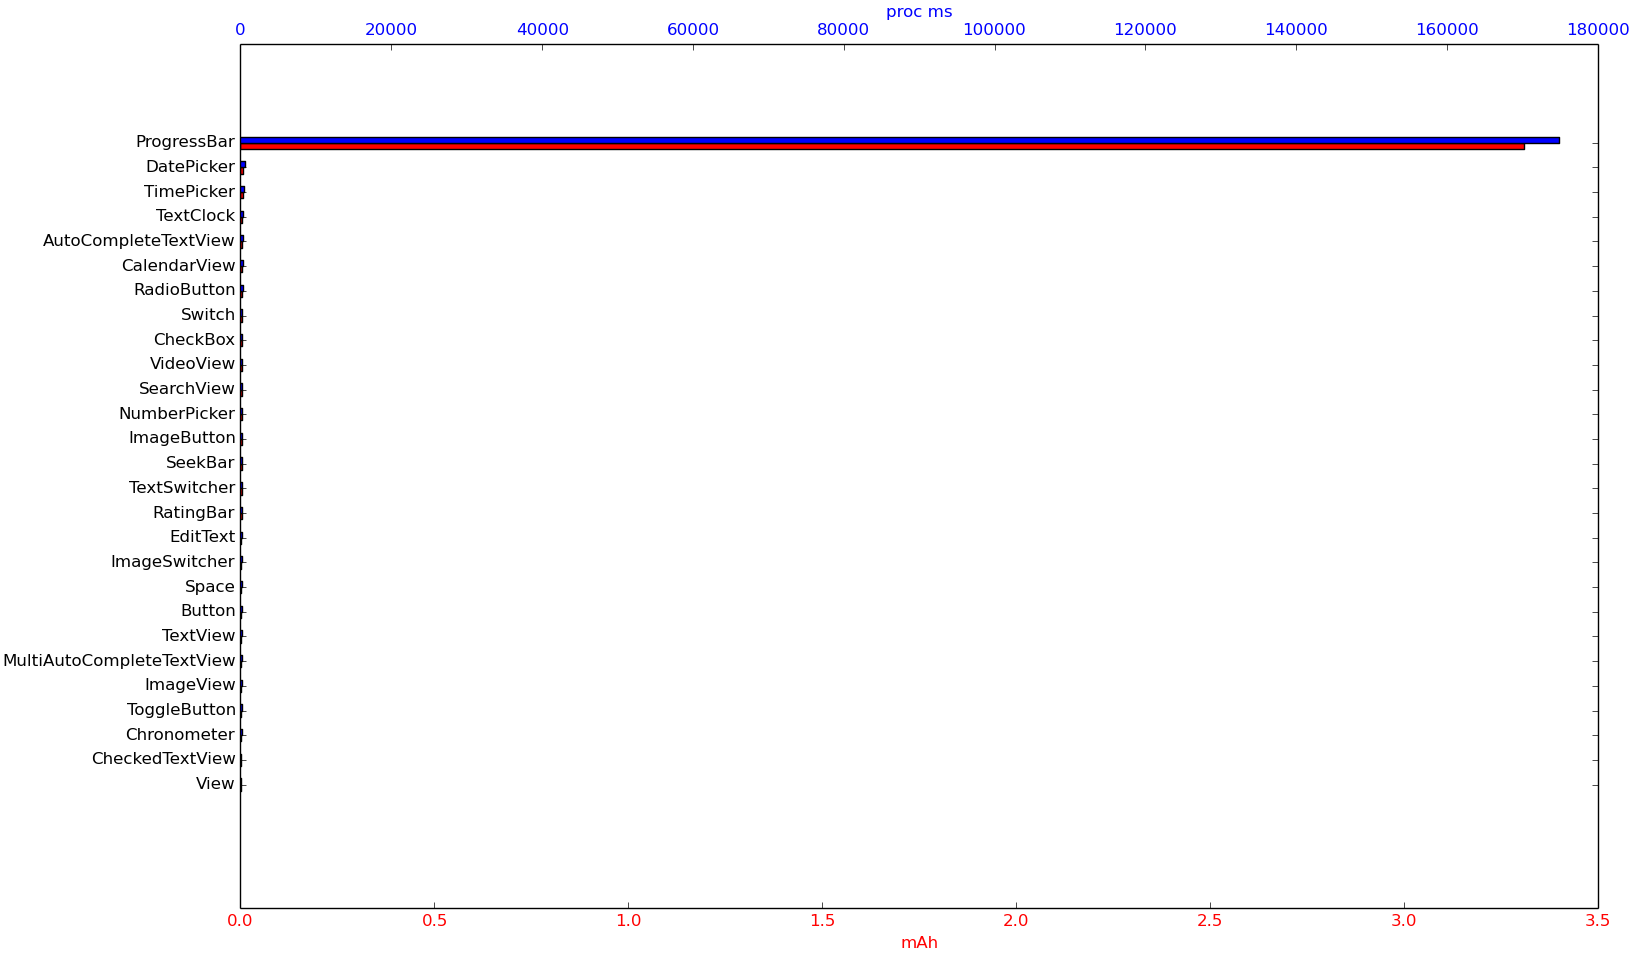
\includegraphics[width=\linewidth]{result}
    \end{frame}
    \begin{frame}
        \frametitle{Результаты измерений}
        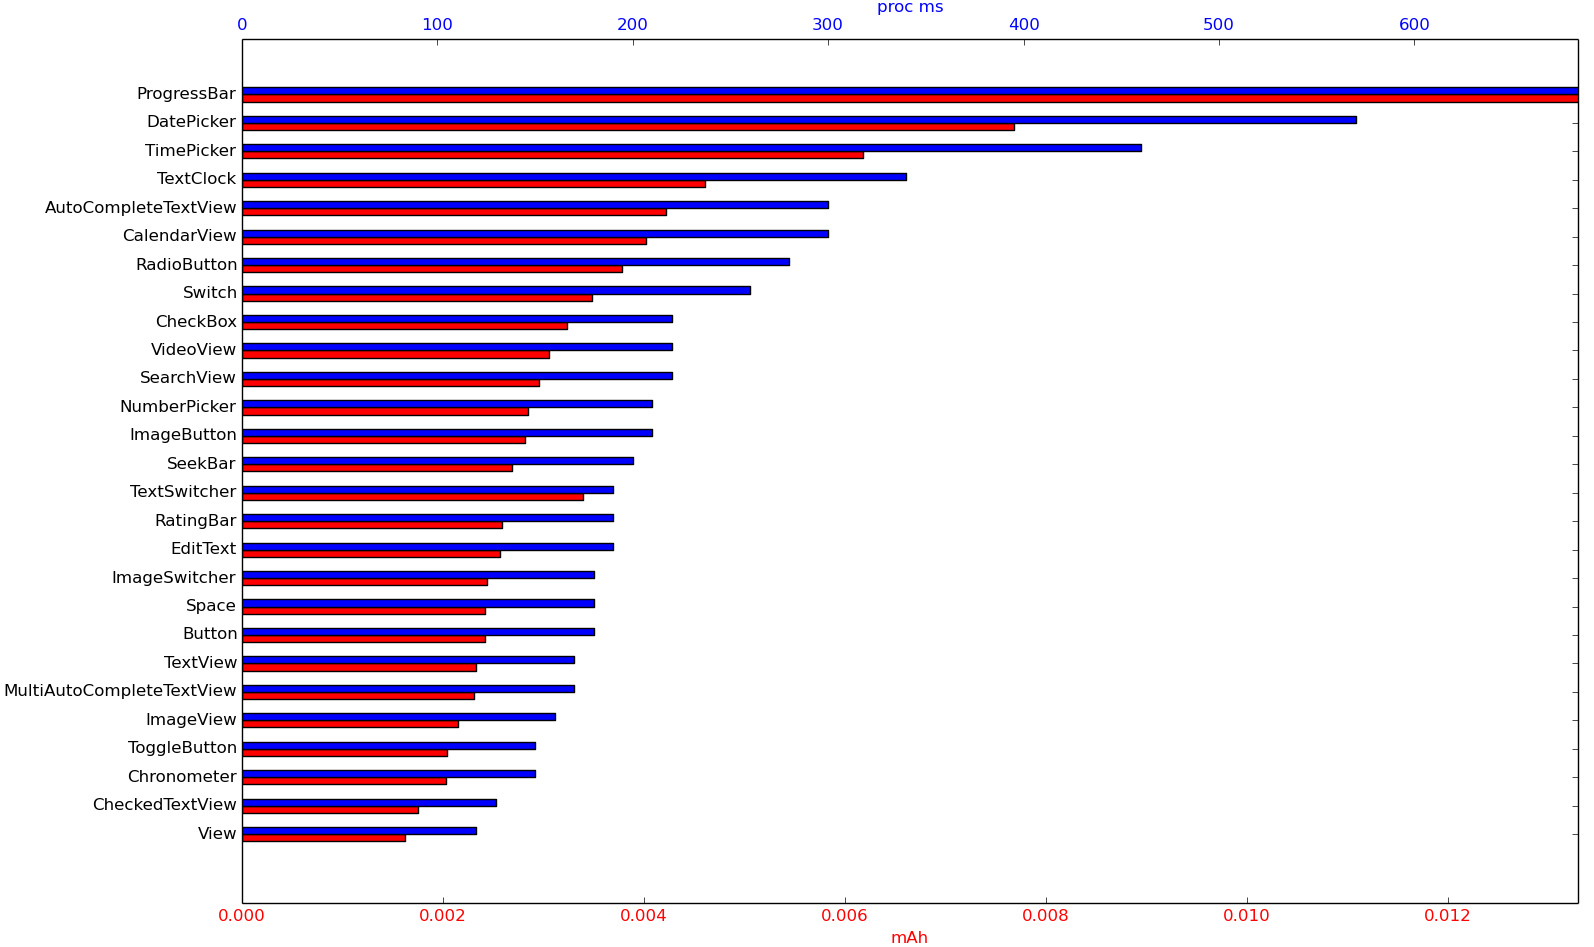
\includegraphics[width=\linewidth]{result_scaled}
    \end{frame}
    \begin{frame}
        \frametitle{Библиотека}
        \framesubtitle{База данных}
        {\scriptsize \begin{multicols}{2}
            \begin{itemize}
                \item ProgressBar --- Switch
                \item DatePicker --- CalendarView
                \item TimePicker --- AutoCompleteTextView
                \item AutoCompleteTextView – EditText
                \item CalendarView --- EditText
                \item RadioButton --- Switch with custom logic
                \item Switch --- CheckBox
                \item CheckBox --- TextSwitcher
                \item SearchView --- EditText
                \item NumberPicker --- SeekBar
                \item ImageButton --- ImageSwitcher
                \item SeekBar --- EditText
                \item TextSwitcher --- ImageSwitcher
                \item RatingBar --- EditText
                \item EditText --- MultiAutoCompleteTextView
                \item ImageSwitcher --- ToggleButton
                \item Space --- View
                \item Button --- TextView
                \item TextView --- ImageView
                \item MultiAutoCompleteTextView --- ToggleButton
                \item ImageView --- CheckedTextView
                \item ToggleButton --- CheckedTextView
                \item CheckedTextView --- View with background
            \end{itemize}
        \end{multicols}}
    \end{frame}
    \begin{frame}
        \frametitle{Библиотека}
        \framesubtitle{Проектирование}
        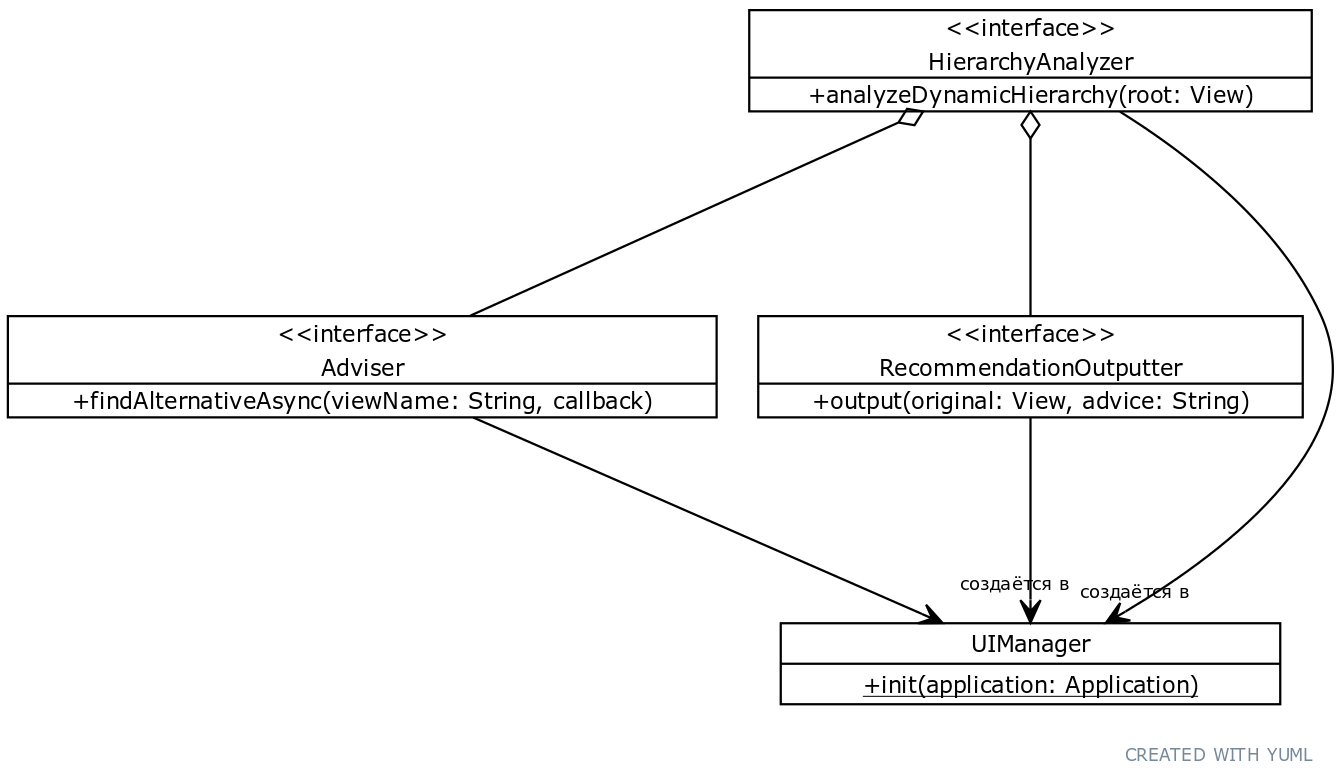
\includegraphics[width=\linewidth]{uml_interfaces}
    \end{frame}
    \begin{frame}
        \frametitle{Итоги работы}
        \centering
        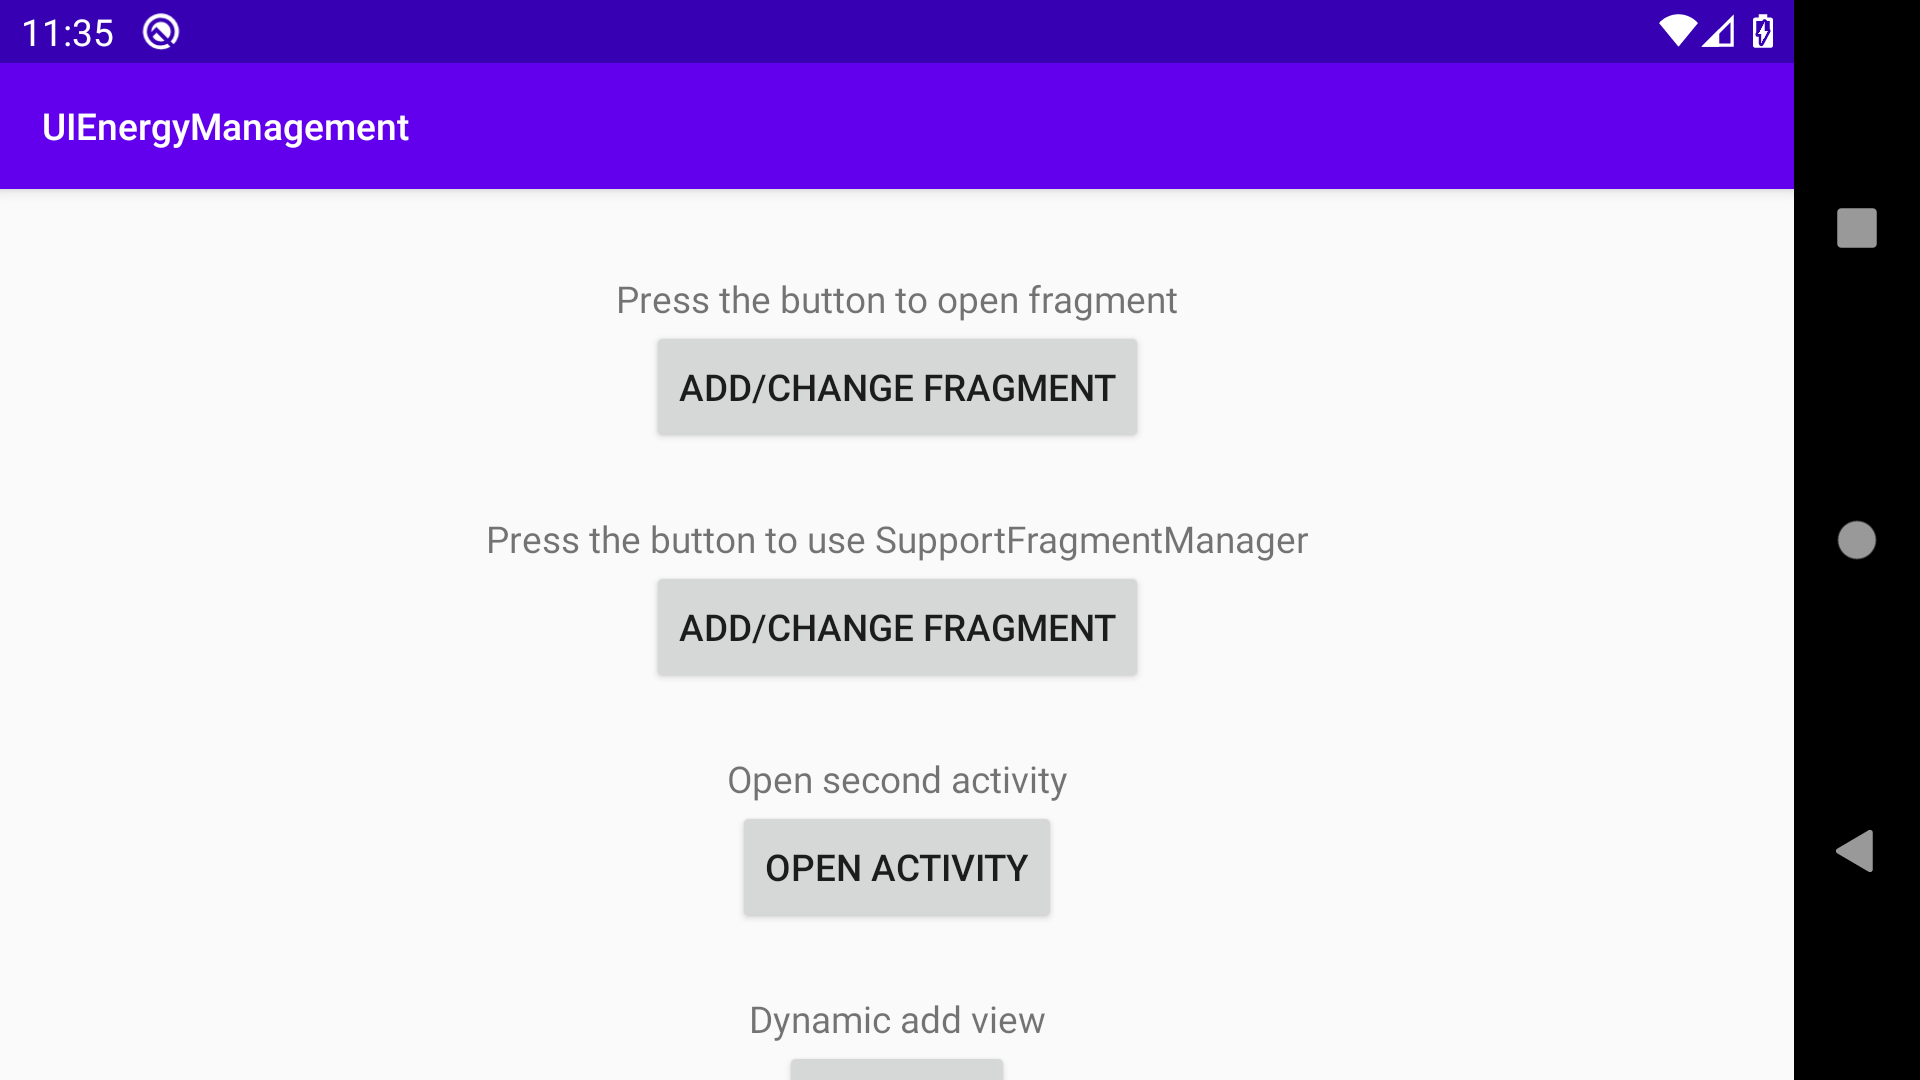
\includegraphics[width=0.8\linewidth]{example}
        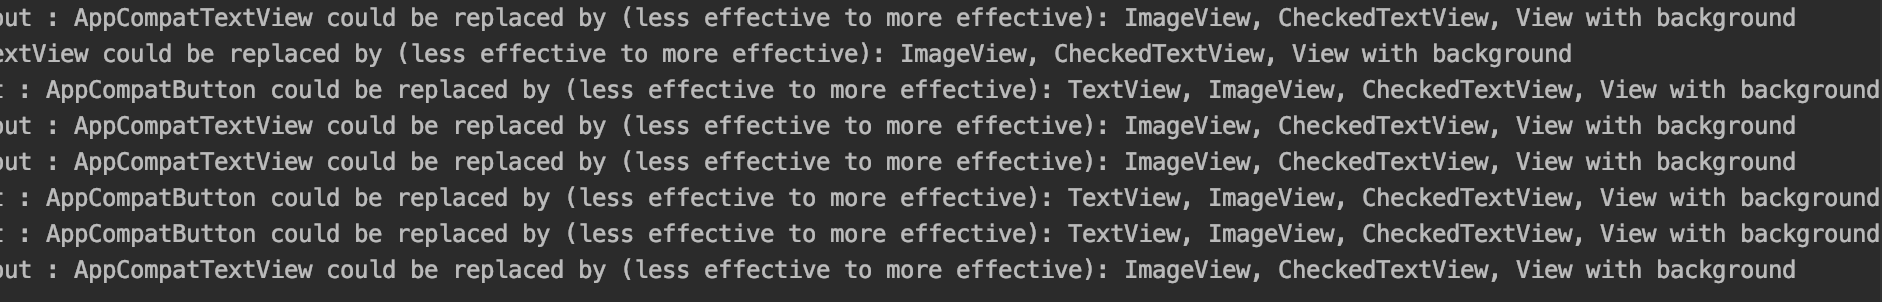
\includegraphics[width=\linewidth]{example_log}
    \end{frame}
    \begin{frame}
        \frametitle{Заключение}
        Сформированная база данных, используется разработанной библиотекой для формирования советов по уменьшению энергопотребления приложения. Это позволит разработчикам получать советы по их оптимизации неэффективных виджетов.\\~
        
        Код и результаты измерений опубликованы на GitHub: https://github.com/Yundin/UIEnergyManagement\\~

        Ограничения:
        \begin{itemize}
            \item Отсутствие доступа к стороннему оборудованию для измерения энергопотребления;
            \item Отсутствие доступа к устройству без сторонних приложений и без служб Google Play Services;
            \item Наличие лишь одного устройства для тестирования.
        \end{itemize}
    \end{frame}
    \begin{frame}
        \frametitle{Перспективы развития}
        В дальнейших исследованиях работа может быть расширена следующим образом:
        \begin{itemize}
            \item Увеличено количество проводимых измерений; 
            \item Виджеты во время тестирования могут перерисовываться вызовом метода invalidate;
            \item Может быть сымитировано пользовательское взаимодействие с устройством.
        \end{itemize}
    \end{frame}
    \begin{frame}[c]
        \begin{center}
            \frametitle{\LARGE Спасибо за внимание!}

            { \LARGE Готов ответить на ваши вопросы. }
        \end{center}
    \end{frame}
\end{document}
